\subsection{Verification and validation}~\\
\noindent \textit{\underline{Belief:}} 
Verification and validation in software development for CS is difficult and strictly scientific \cite{carver07_environment, kanewala13_testing, carver06_hpc, Prabhu11_cssurvey, basili08_hpc}.

\noindent \textit{\underline{Rationale:}} 
According to Carver et al.~\cite{carver07_environment},
CS verification means ensuring the mathematical model matches the real world; while CS validation means ensure the computational model matches the mathematical model  Past studies argued that verification and validation of scientific software
should be  difficult for  several reasons:

\bi
    \item Lack of suitable test oracles \cite{kanewala13_testing},
    \item Complex distributed hardware environments with no comparable software \cite{basili08_hpc},
    \item Scientists often suspect that the problems of the software is the results of their scientific theory~\cite{faulk09_secs},
    \item Lack of physical experimentation and experimental validation is impractical \cite{carver07_environment}. 
\ei

\noindent \textit{\underline{Modeling Assumptions:}} See  above, in \S\ref{model}

\noindent \textit{\underline{Prediction:}}
Verification and validation in CS
``difficult'' if the observed CS effort in this area
is much larger than some known baseline.  As to ``strictly scientific'', we should see far more ``scientific
enhancements'' that otherwise (e.g. ``bug fixes'' plus ``engineering enhancement''). 

\noindent \textit{\underline{Result:}}
It is easy to show that CS software verification and validation is heavily  focused on scientific issues.
Table \ref{tbl:testing} shows that ``scientific testing'' is the largest type of commit in our labeled Testing commits sample (at 45\%).  Far less effort is spend on ``engineering testing'' (only 17\%). 


As to showing the CS verification and validation is ``more difficult'',
the Table \ref{tbl:everything} should be compared to Figure \ref{fig:SE_activities}, which shows the 85\% percent  of commits in standard SE projects
 associated with bug fixes and enhancements.  This data comes from a recent study of the top-20 highly starred from Github that satisfy our sanity checks of Table~\ref{tbl:sanity} \footnote{TBD:need more data. 20 se projects}.
Since 85\% is much larger than 22\%, we conclude that, for verification and validation, 
far less effort is being spent in CS projects than SE.

\begin{figure}
     \centering
     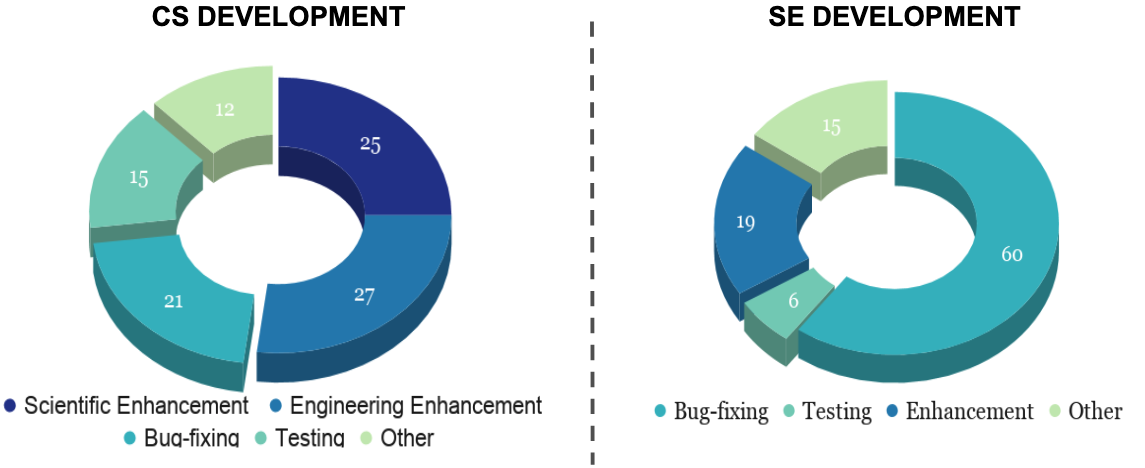
\includegraphics[width=\linewidth]{img/development.png} 
     \caption{Distribution of development activities within CS (left) and SE (right) projects within our sample.}
     \label{fig:SE_activities}
 \end{figure}


\begin{table}[!t]
\caption{Labels of testing type commits from the labeled Testing commits.}\label{tbl:testing}


\vspace{3mm}

\begin{center}
%\begin{threeparttable}
%\vspace{-10pt}
%\resizebox{!}{0.2\linewidth}{
%\setlength        abcolsep{10pt}
\vspace{-10pt}\begin{tabular}{l|c|c}
 \multicolumn{1}{c|}{} & \multicolumn{1}{c|}{Absolute} & \multicolumn{1}{c}{Percentage}\\
\hline
Science & 29 & 45\% \\
Engineering & 11 & 17\% \\
Other & 25 & 38\% 
\end{tabular}
%}
%\end{threeparttable}
\end{center}
\vspace{3mm}
\end{table}



% Among all the defects fixing, the scientific and engineering defects are at the same rate. Yet, the testing focuses solely on scientific aspect, almost three times (45\%/17\%), more than engineering testing. In a sense, scientists solely believe that the software is defected due to their science understanding when transferring that to source code while overlooking the engineering aspect. Yet, it is understandable because scientists have a lot of responsibilities (read and write papers, grants, give presentations, develop scientific models, etc) so they can only focus on testing on what they good at, i.e. scientific models. It is possibly useful for the community to incorporate automated SE testing tools for CS projects. 

\noindent \textit{\underline{Conclusion:}}
We endorse the belief that CS V\&V is mostly concerned with scientific issues. But since CS V\&V requires fewer commits
that SE projects, we cannot endorse a belief that 
verification and validation in software development for CS is more difficult than in other disciplines.

\noindent \textit{\underline{Discussion:}}
This result is somewhat strange since it runs counter to standard beliefs in the SE literature (e.g. Brookes argues that unit tests and systems tests will consume half the time of any project~\cite{brooks1995mythical}).
We conjecture that the larger V\&V effort in SE  is due to the nature of CS problems.  CS software is more grounded in unchanging physical realities that standard SE software:
\bi
\item
CS software is written to correspond to physical phenomena, the nature of which may never change (e.g. the atomic weight of iron).
\item
On the other hand, standard SE software (e.g. the highly starred projects in Github) is written to correspond to an ever-changing ecology of platforms, tools, user expectations, and newly-arrive AI algorithms, etc etc.   
Hence, it is not surprising  SE software requires more verification and validation effort than CS software since the problem it addresses are more dynamic.
\ei

Whatever the reason, 
note that this result calls for a different kind of testing device in CS.  In standard SE, a ``test'' can be something as simple as a unit test (checking if, for example, that subtrees remain in sorted order after insertion).
But in CS, ``tests'' need to be a higher level and refer back to some core physical properties as defined
by scientific theory.  